% Copyright 2004 by Till Tantau <tantau@users.sourceforge.net>.
%
% In principle, this file can be redistributed and/or modified under
% the terms of the GNU Public License, version 2.
%
% However, this file is supposed to be a template to be modified
% for your own needs. For this reason, if you use this file as a
% template and not specifically distribute it as part of a another
% package/program, I grant the extra permission to freely copy and
% modify this file as you see fit and even to delete this copyright
% notice. 

\documentclass{beamer}
\usepackage[utf8]{inputenc}
\usepackage[brazilian]{babel}

% There are many different themes available for Beamer. A comprehensive
% list with examples is given here:
% http://deic.uab.es/~iblanes/beamer_gallery/index_by_theme.html
% You can uncomment the themes below if you would like to use a different
% one:
%\usetheme{AnnArbor}
%\usetheme{Antibes}
%\usetheme{Bergen}
%\usetheme{Berkeley}
%\usetheme{Berlin}
%\usetheme{Boadilla}
%\usetheme{boxes}
\usetheme{CambridgeUS}
%\usetheme{Copenhagen}
%\usetheme{Darmstadt}
%\usetheme{default}
%\usetheme{Frankfurt}
%\usetheme{Goettingen}
%\usetheme{Hannover}
%\usetheme{Ilmenau}
%\usetheme{JuanLesPins}
%\usetheme{Luebeck}
%\usetheme{Madrid}
%\usetheme{Malmoe}
%\usetheme{Marburg}
%\usetheme{Montpellier}
%\usetheme{PaloAlto}
%\usetheme{Pittsburgh}
%\usetheme{Rochester}
%\usetheme{Singapore}
%\usetheme{Szeged}
%\usetheme{Warsaw}

\title{Distros - Unix}

% A subtitle is optional and this may be deleted
\subtitle{Curso de Unix}

\author{PET Computação}
% - Give the names in the same order as the appear in the paper.
% - Use the \inst{?} command only if the authors have different
%   affiliation.

\institute[UFSC] % (optional, but mostly needed)
{
%
  Departamento de Informática e Estatística\\
  Universidade de Santa Catarina}
% - Use the \inst command only if there are several affiliations.
% - Keep it simple, no one is interested in your street address.

\date{PET Computação, 2015}
% - Either use conference name or its abbreviation.
% - Not really informative to the audience, more for people (including
%   yourself) who are reading the slides online

\subject{Curso de Unix}
% This is only inserted into the PDF information catalog. Can be left
% out. 

% If you have a file called "university-logo-filename.xxx", where xxx
% is a graphic format that can be processed by latex or pdflatex,
% resp., then you can add a logo as follows:

% \pgfdeclareimage[height=0.5cm]{university-logo}{university-logo-filename}
% \logo{\pgfuseimage{university-logo}}

% Delete this, if you do not want the table of contents to pop up at
% the beginning of each subsection:
\AtBeginSubsection[]
{
  \begin{frame}<beamer>{Sumário}
    \tableofcontents[currentsection,currentsubsection]
  \end{frame}
}

% Let's get started
\begin{document}

\begin{frame}
  \titlepage
\end{frame}

\begin{frame}{Sumário}
  \tableofcontents
  % You might wish to add the option [pausesections]
\end{frame}

% Section and subsections will appear in the presentation overview
% and table of contents.
\section{Distribuições de Linux}

\subsection{Amigáveis}

\begin{frame}{Ubuntu}
    \begin{itemize}
        \item{Ubuntu é, atualmente, a distro mais popular de Linux}
        \item{Baseado em Debian}
        \item{Usa dpkg e APT como gerenciamento de pacotes}
        \item{Tem Unity como ambiente padrão}
        \item{Possui variações como Kubuntu (KDE), Xubuntu (XFCE4) e Lubuntu (LXDE)}
        \item{É patrocinado pela Canonical Ltd.}
    \end{itemize}
    \begin{figure}[h!]
        \centering
        
\includegraphics[scale=0.25]{ubuntu.png}
    \end{figure}
\end{frame}

\begin{frame}{Ubuntu}{Ubuntu}
 \begin{figure}[h!]
        \centering
        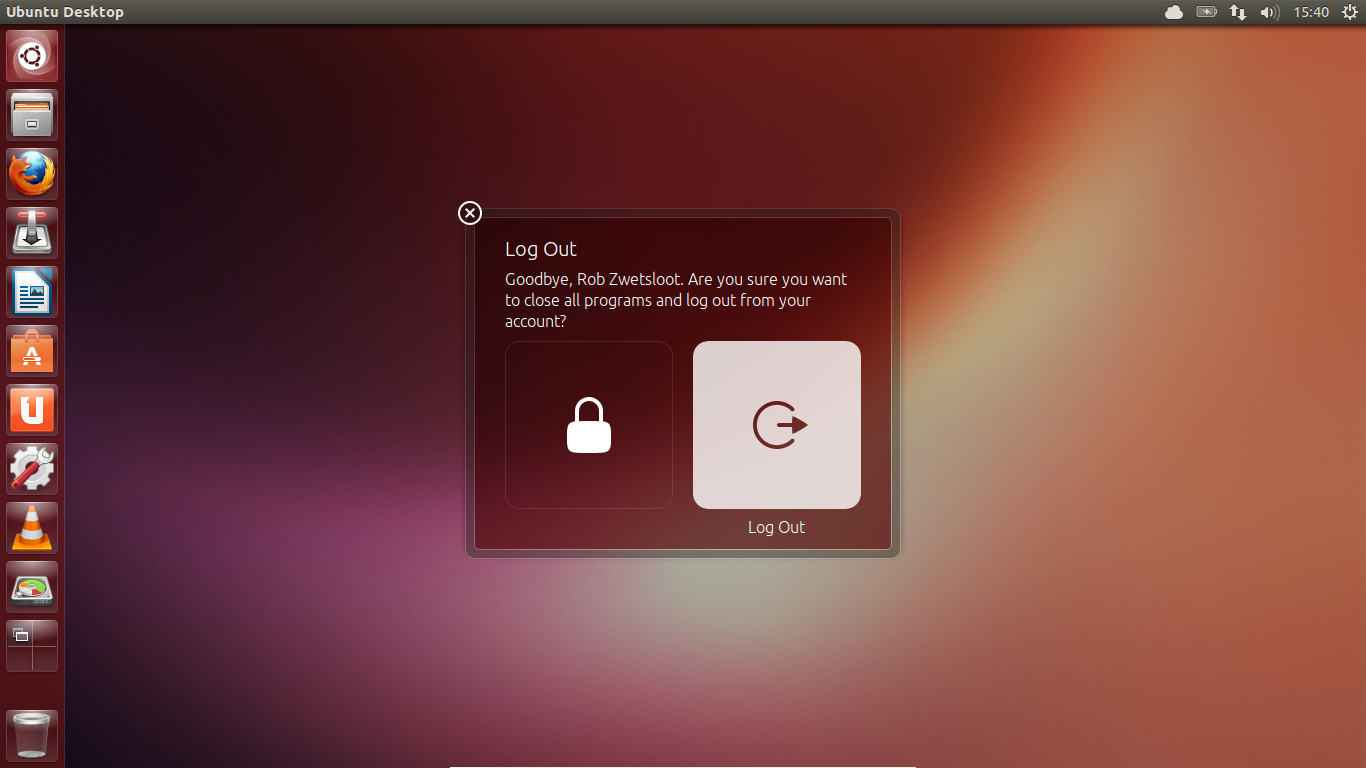
\includegraphics[scale=0.16]{unit.png}
        \caption{Ubuntu com Interface gráfica Unity (padrão)}
        \label{fig:Comando ls}
    \end{figure}
\end{frame}

\begin{frame}{Ubuntu}{Kubuntu}
 \begin{figure}[h!]
        \centering
        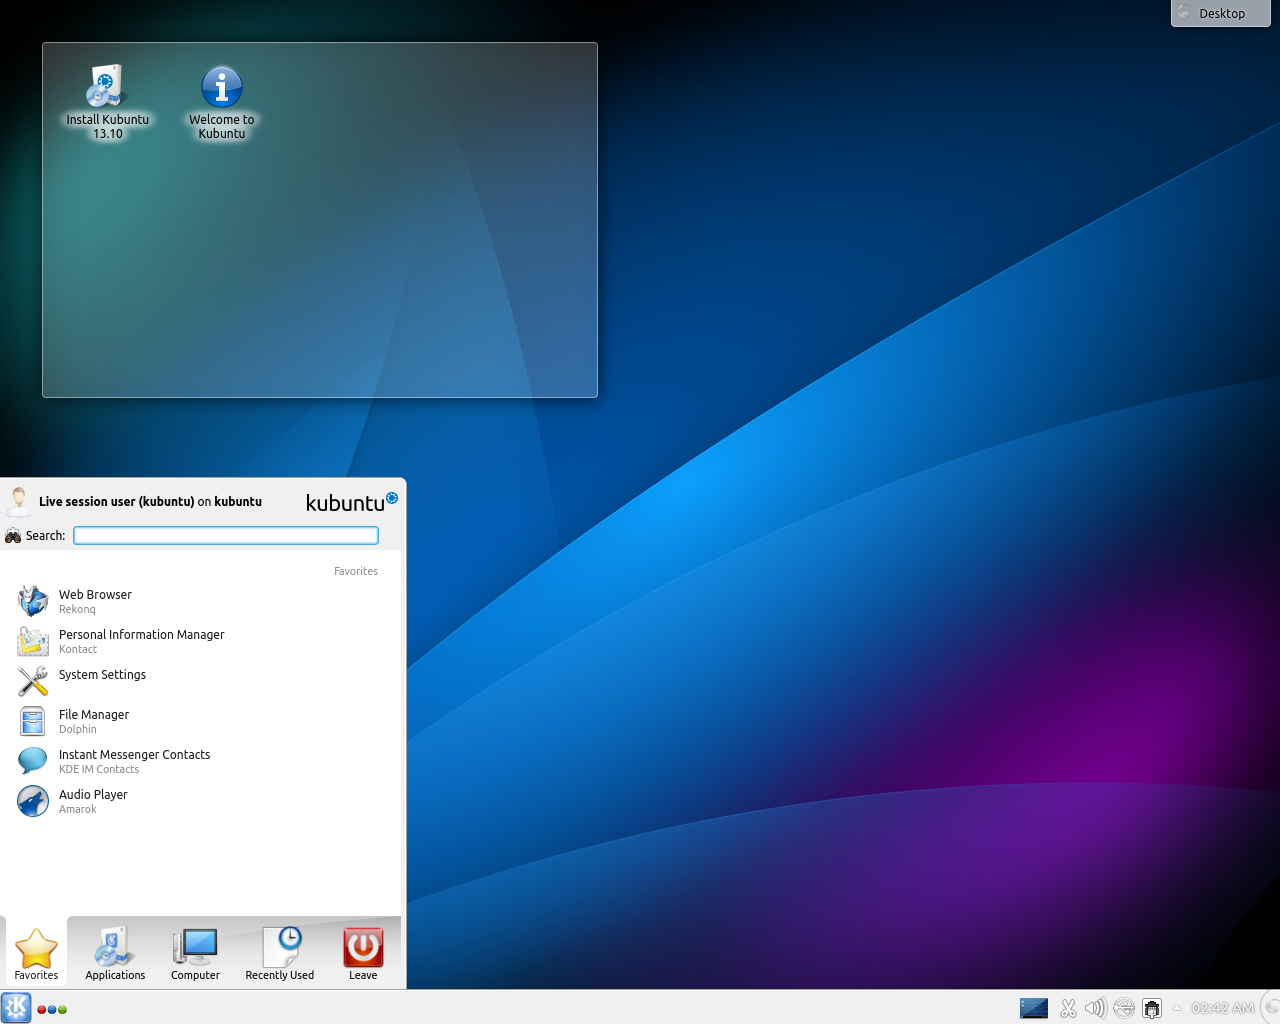
\includegraphics[scale=0.20]{Kubuntu.png}
        \caption{Ubuntu com Interface gráfica KDE}
        \label{fig:Comando ls}
    \end{figure}
\end{frame}

\begin{frame}{Ubuntu}{Xubuntu}
 \begin{figure}[h!]
        \centering
        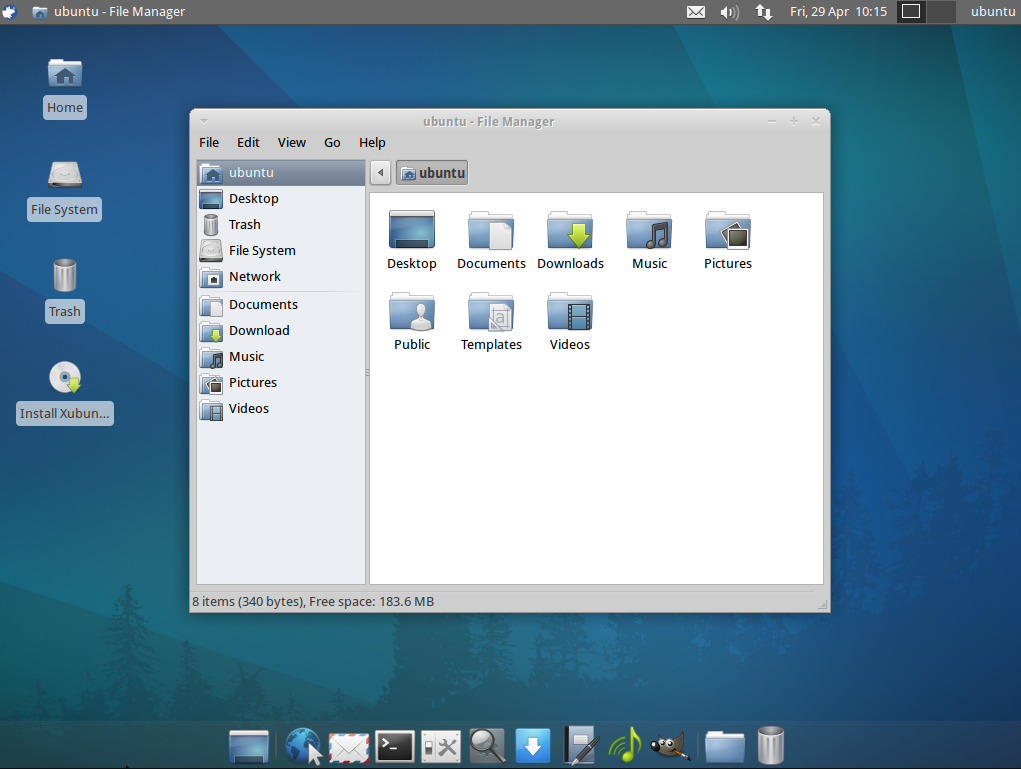
\includegraphics[scale=0.20]{Xubuntu.png}
        \caption{Ubuntu com Interface gráfica XFCE4}
        \label{fig:Comando ls}
    \end{figure}
\end{frame}

\begin{frame}{Ubuntu}{Lubuntu}
 \begin{figure}[h!]
        \centering
        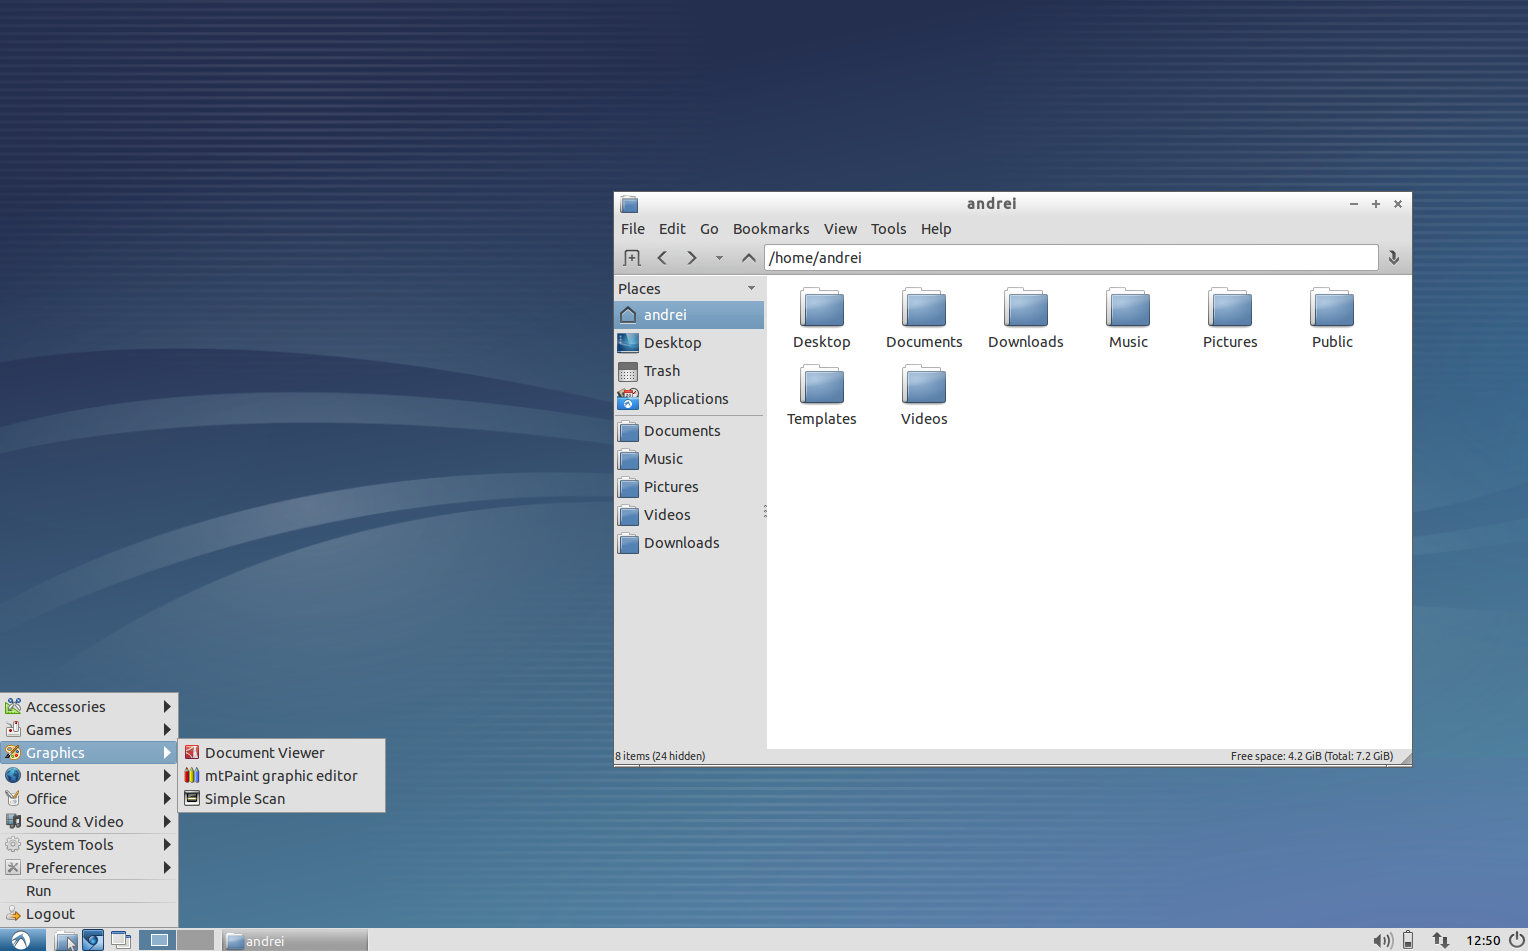
\includegraphics[scale=0.16]{lubuntu.png}
        \caption{Ubuntu com Interface gráfica LXDE}
        \label{fig:Comando ls}
    \end{figure}
\end{frame}

\begin{frame}{Linux Mint}
    \begin{itemize}
        \item{Famoso por ser muito amigável}
        \item{Linux Mint é, atualmente, a distro que mais cresce em usuários}
        \item{Baseado em Ubuntu}
        \item{Seu objetivo é vir pronta, sem necessidade de instalar mais nada}
        \item{Usa dpkg e APT como gerenciamento de pacotes}
        \item{Possui versões com Cinnamon (padrão), MATE, XFCE e KDE como ambiente}
    \end{itemize}
    \begin{figure}[h!]
        \centering
        
\includegraphics[scale=0.10]{mint.png}
    \end{figure}
\end{frame}


\begin{frame}{Mint}{Cinnamon (padrão)}
 \begin{figure}[h!]
        \centering
        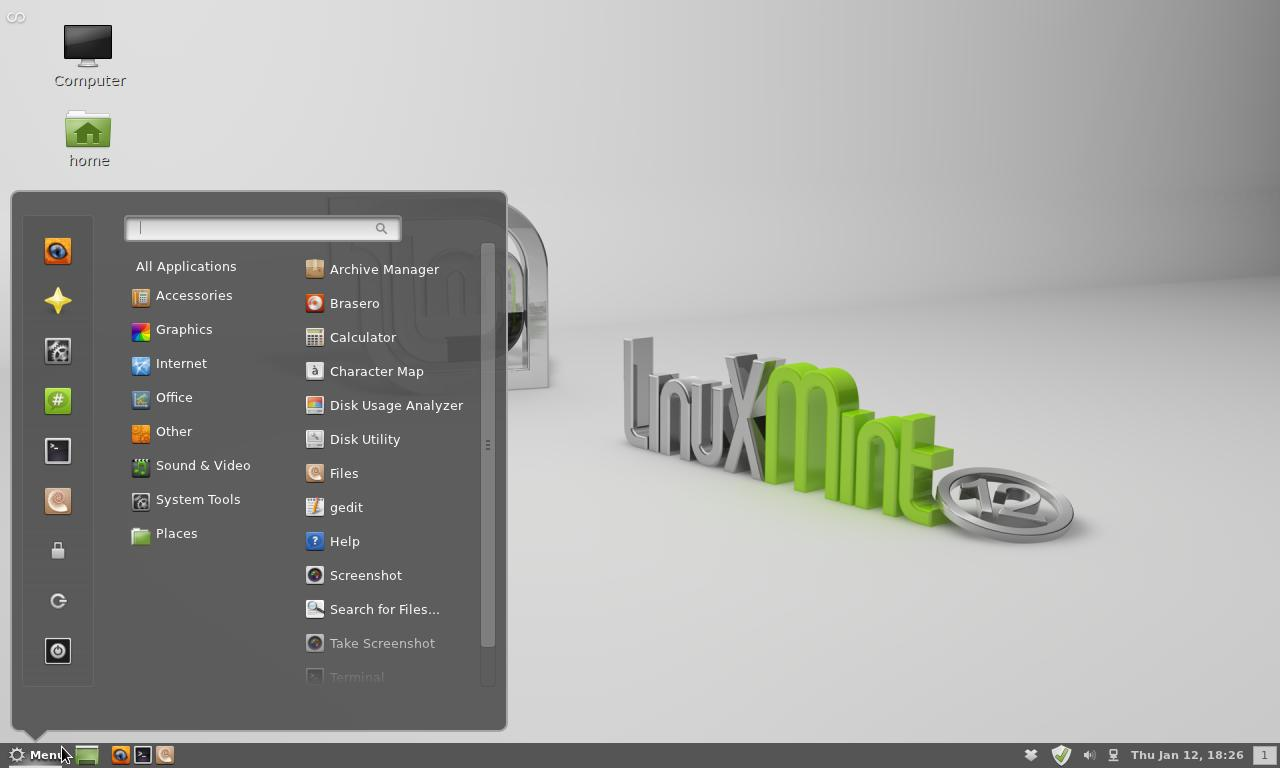
\includegraphics[scale=0.20]{MintCinnamon.jpg}
        \caption{Mint com Interface gráfica Cinnamon (padrão)}
        \label{fig:Comando ls}
    \end{figure}
\end{frame}

\begin{frame}{Mint}{Mate}
 \begin{figure}[h!]
        \centering
        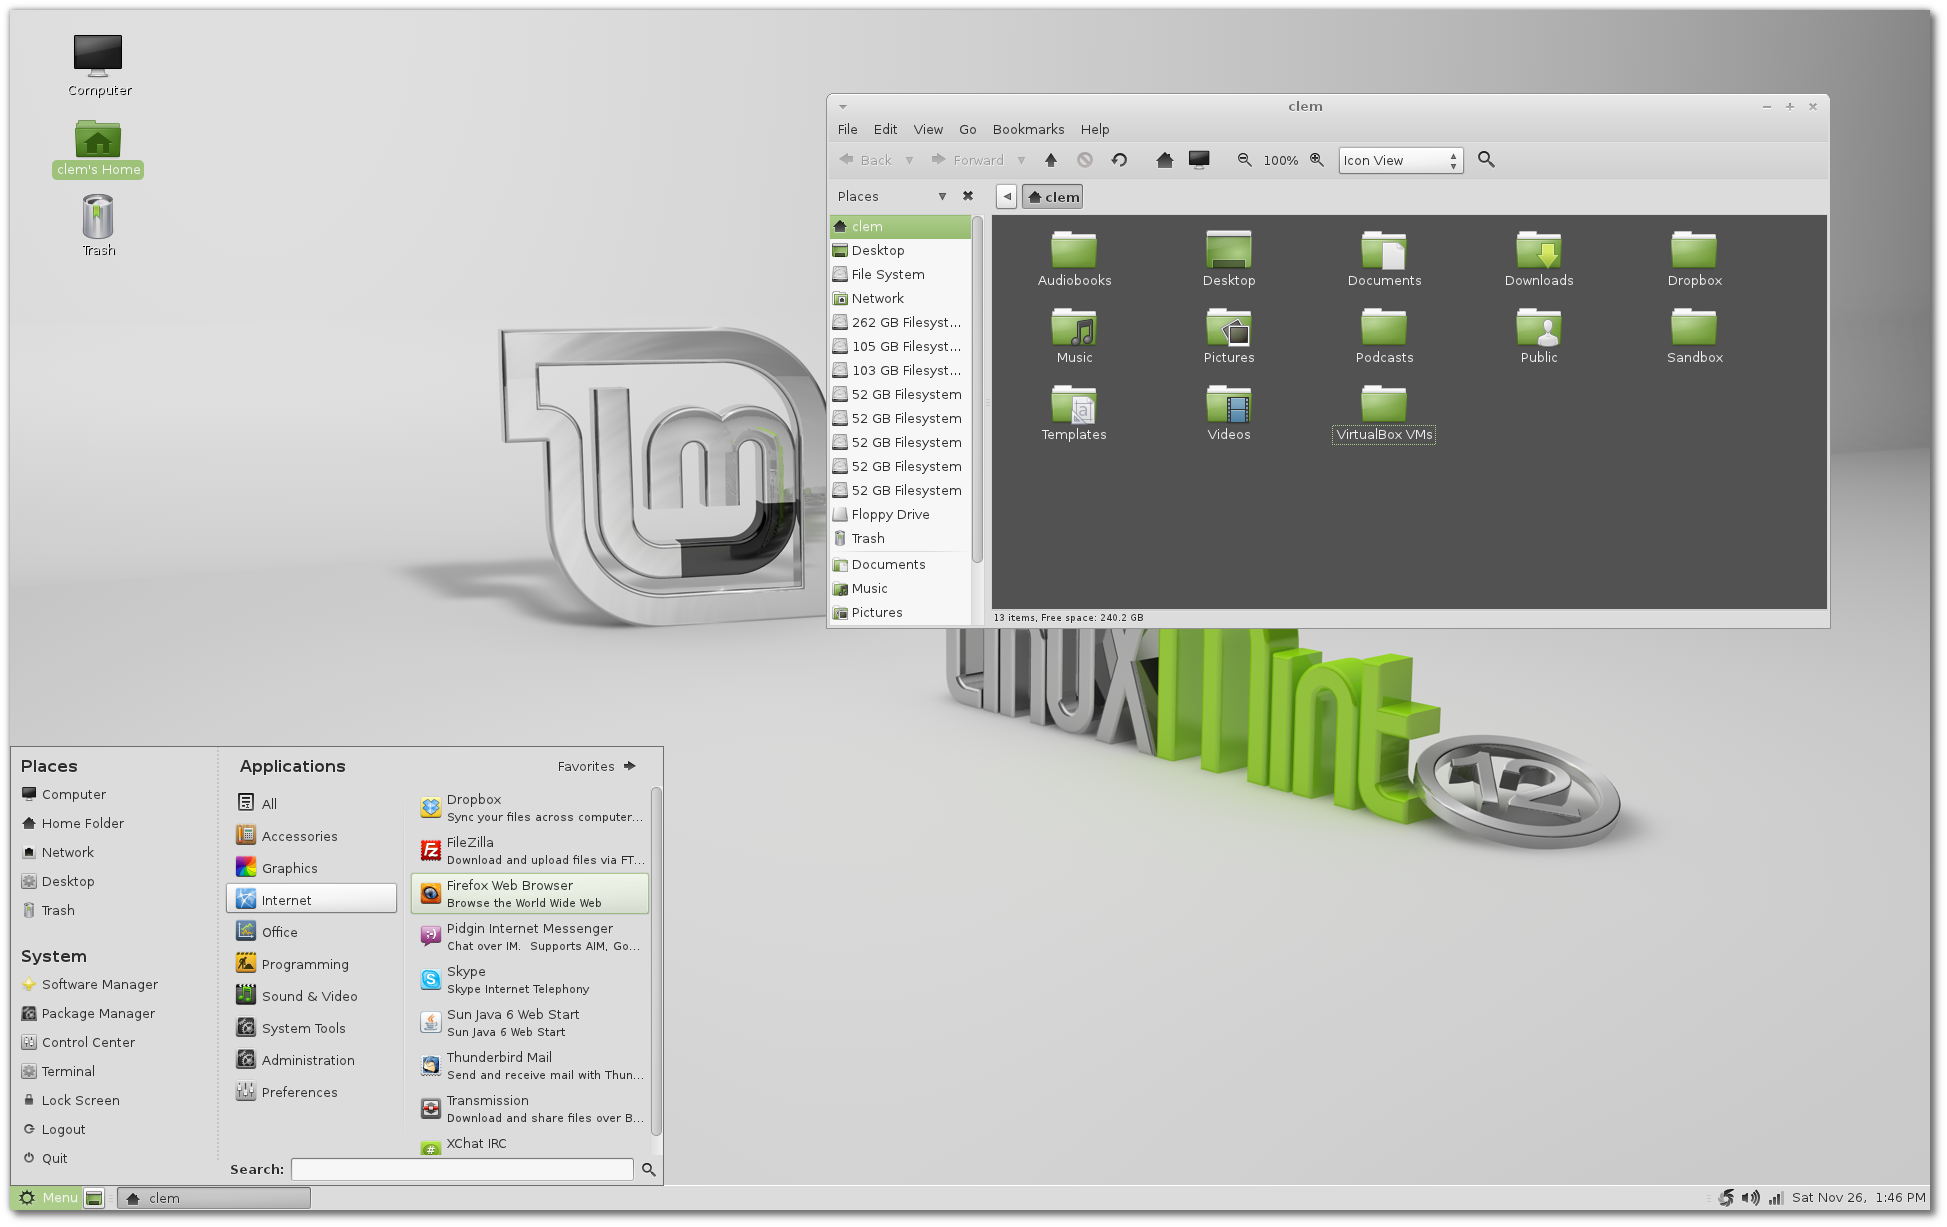
\includegraphics[scale=0.12]{MintMate.png}
        \caption{Mint com Interface gráfica Mate}
        \label{fig:Comando ls}
    \end{figure}
\end{frame}

\begin{frame}{Mint}{XFCE}
 \begin{figure}[h!]
        \centering
        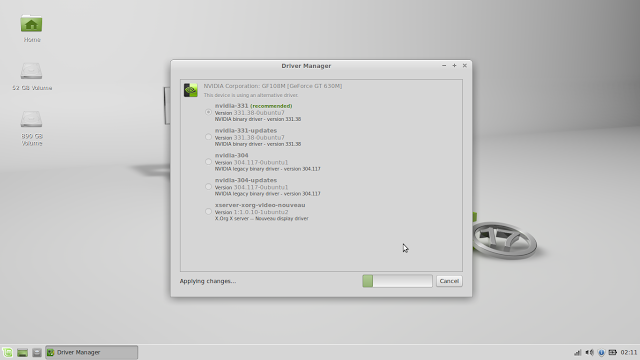
\includegraphics[scale=0.4]{MintXFCE.png}
        \caption{Mint com Interface gráfica XFCE}
        \label{fig:Comando ls}
    \end{figure}
\end{frame}

\begin{frame}{Fedora}
    \begin{itemize}
        \item{Foi uma das primeiras distros amigáveis, sendo criada em 1994 como \textbf{Red Hat Linux}}
        \item{Já foi a distro mais utilizada antes do Ubuntu}
        \item{É completamente livre e gratuita por padrão, além de ser atualizada}
        \item{Usa rpm e YUM como gerenciamento de pacotes}
        \item{Possui versões para computadores pessoais (com GNOME), para servidores e computação em nuvem}
    \end{itemize}
    \begin{figure}[h!]
        \centering
        
\includegraphics[scale=0.42]{fedora.png}
    \end{figure}
\end{frame}

\begin{frame}{Fedora}{GNOME (padrão)}
 \begin{figure}[h!]
        \centering
        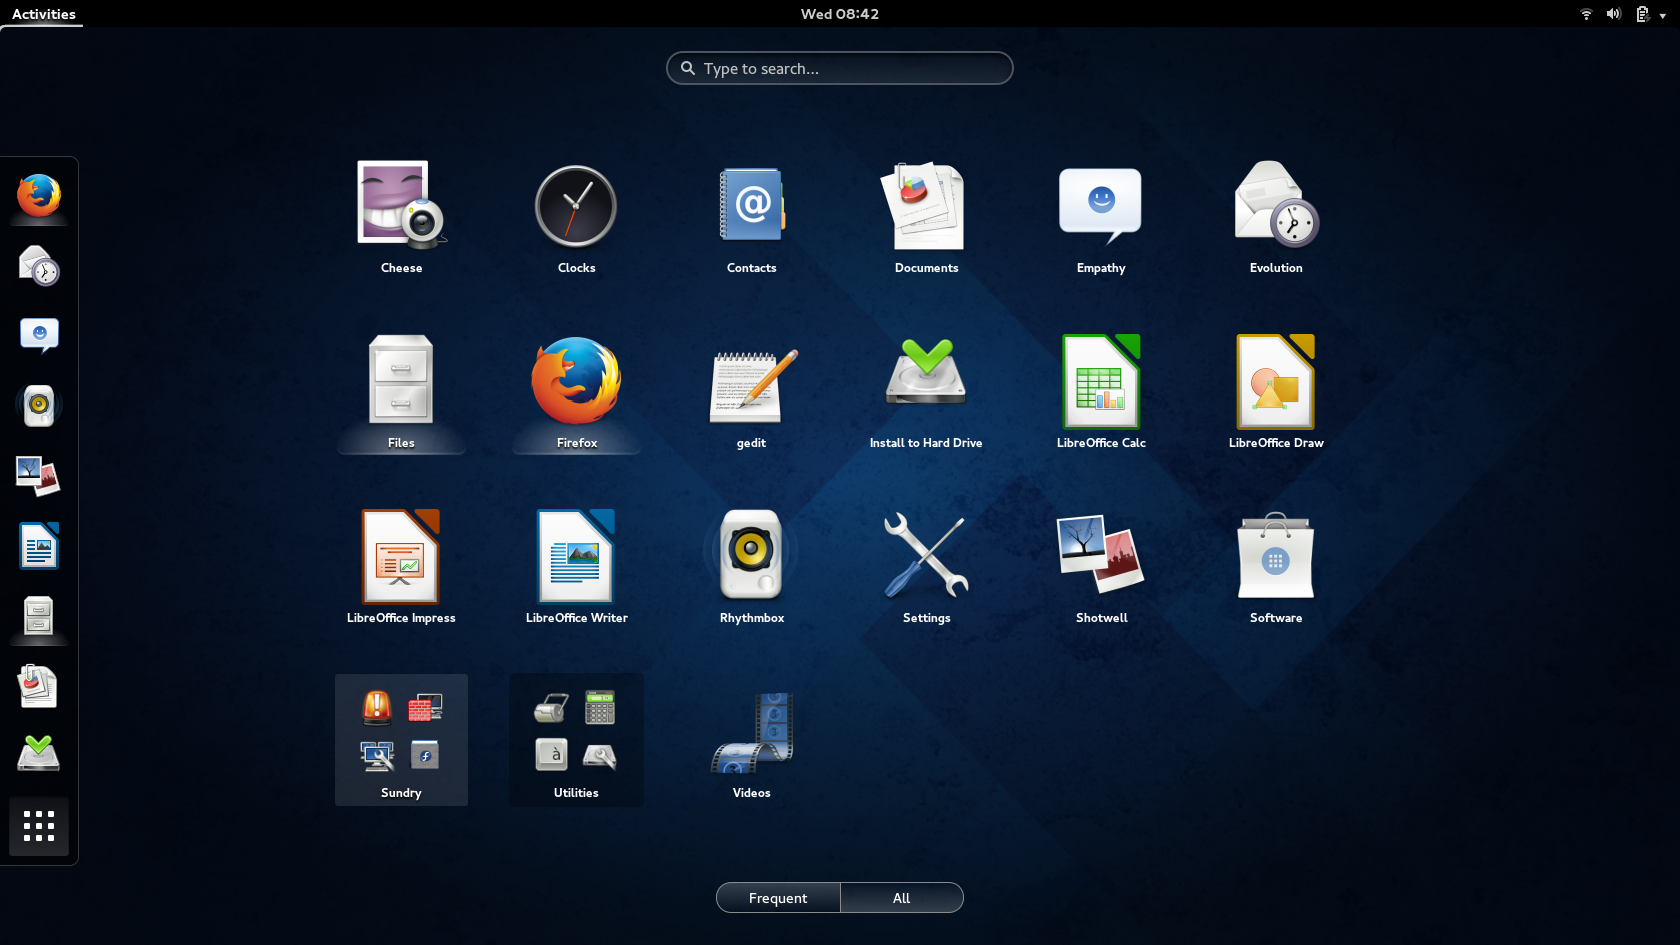
\includegraphics[scale=0.16]{fedoraGNOME.png}
        \caption{Fedora com Interface gráfica GNOME (padrão)}
        \label{fig:Comando ls}
    \end{figure}
\end{frame}

\begin{frame}{Fedora}{KDE}
 \begin{figure}[h!]
        \centering
        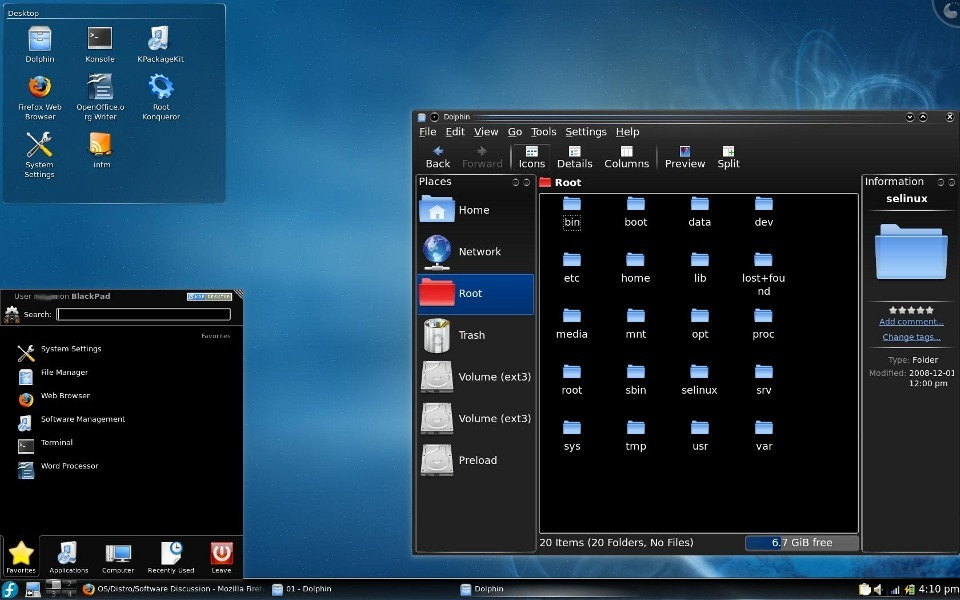
\includegraphics[scale=0.48]{FedoraKDE.jpg}
        \caption{Fedora com Interface gráfica KDE}
        \label{fig:Comando ls}
    \end{figure}
\end{frame}

\begin{frame}{Fedora}{LXDE}
 \begin{figure}[h!]
        \centering
        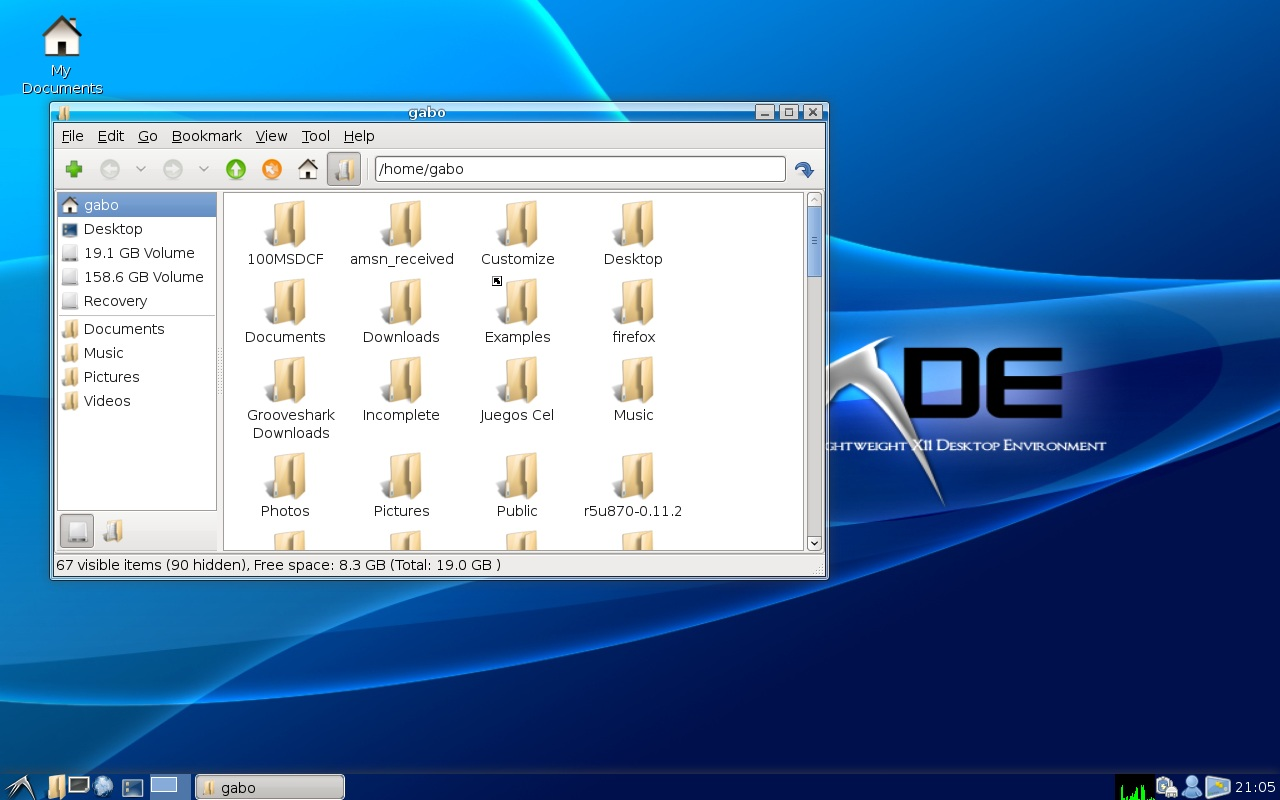
\includegraphics[scale=0.3]{FedoraLXDE.jpg}
        \caption{Fedora com Interface gráfica LXDE}
        \label{fig:Comando ls}
    \end{figure}
\end{frame}

\begin{frame}{Fedora}{XFCE}
 \begin{figure}[h!]
        \centering
        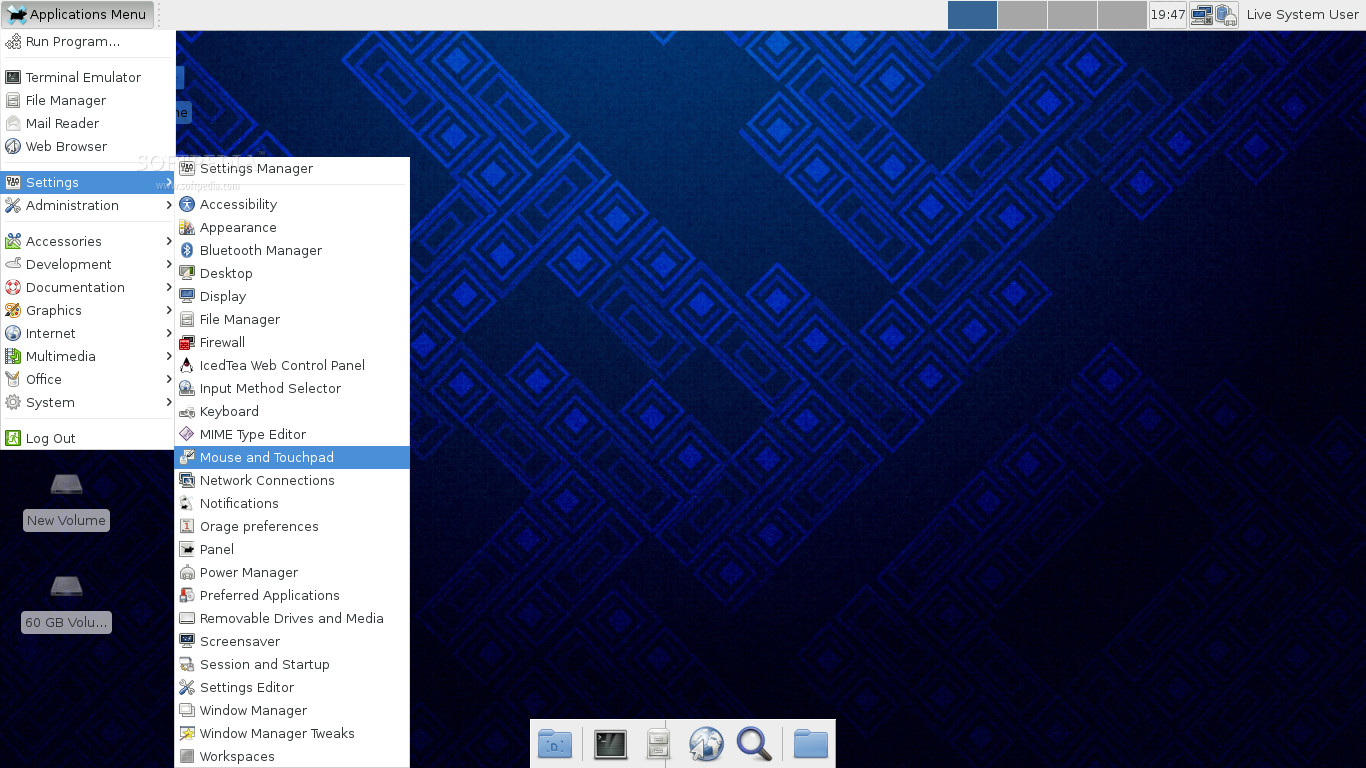
\includegraphics[scale=0.22]{FedoraXFCE.jpg}
        \caption{Fedora com Interface gráfica XFCE}
        \label{fig:Comando ls}
    \end{figure}
\end{frame}

\subsection{Enxutas}

\begin{frame}{Debian}
    \begin{itemize}
        \item{Conhecido por sua estabilidade e compatibilidade com diversas arquiteturas de processadores} 
        \item{É a distro mais utilizada em servidores, com folga}
        \item{Usado como base para mais de 120 distros}
        \item{É completamente livre, porém não é atualizada como o Fedora}
        \item{Usa dpkg e APT como gerenciamento de pacotes}
        \item{Possui versões com GNOME e KDE como ambiente}
    \end{itemize}
    \begin{figure}[h!]
        \centering
        
\includegraphics[scale=0.20]{debian.png}
    \end{figure}
\end{frame}

\begin{frame}{Debian}{GNOME}
 \begin{figure}[h!]
        \centering
        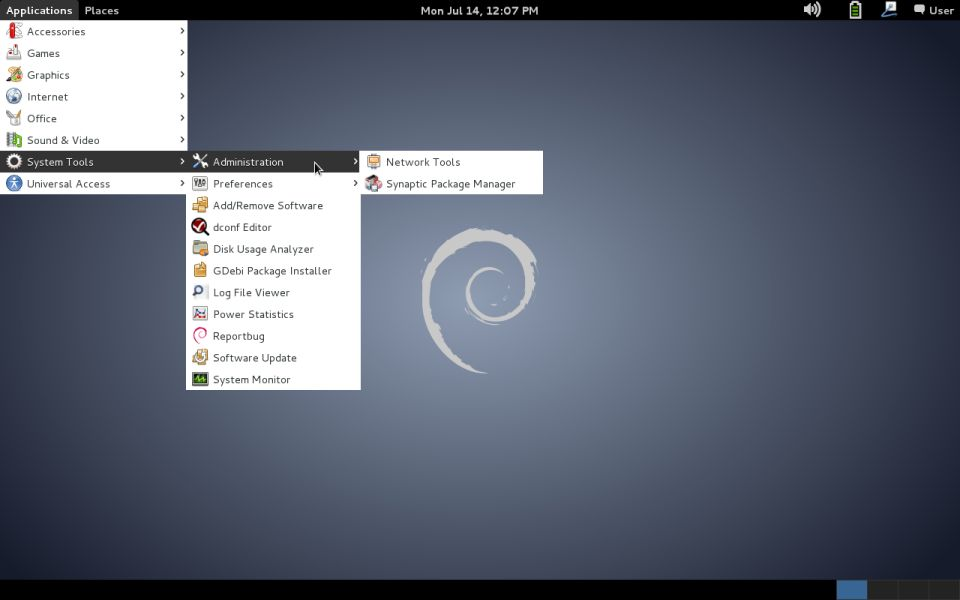
\includegraphics[scale=0.27]{debianGNOME.jpg}
        \caption{Debian com interface gráfica GNOME}
        \label{fig:Comando ls}
    \end{figure}
\end{frame}

\begin{frame}{Manjaro Linux}
    \begin{itemize}
        \item{Baseado em Arch Linux}
        \item{Criado para precisar de menos intervenção do usuário}
        \item{Possui um instalador amigável e ferramentas de detecção de hardware}
        \item{Usa pacman como gerenciamento de pacotes, podendo também utilizar o AUR}
        \item{Possui versões com Openbox e XFCE como ambiente}
    \end{itemize}
    \begin{figure}[h!]
        \centering
        
\includegraphics[scale=0.80]{manjaro.png}
    \end{figure}
\end{frame}

\begin{frame}{Manjaro}{Openbox}
 \begin{figure}[h!]
        \centering
        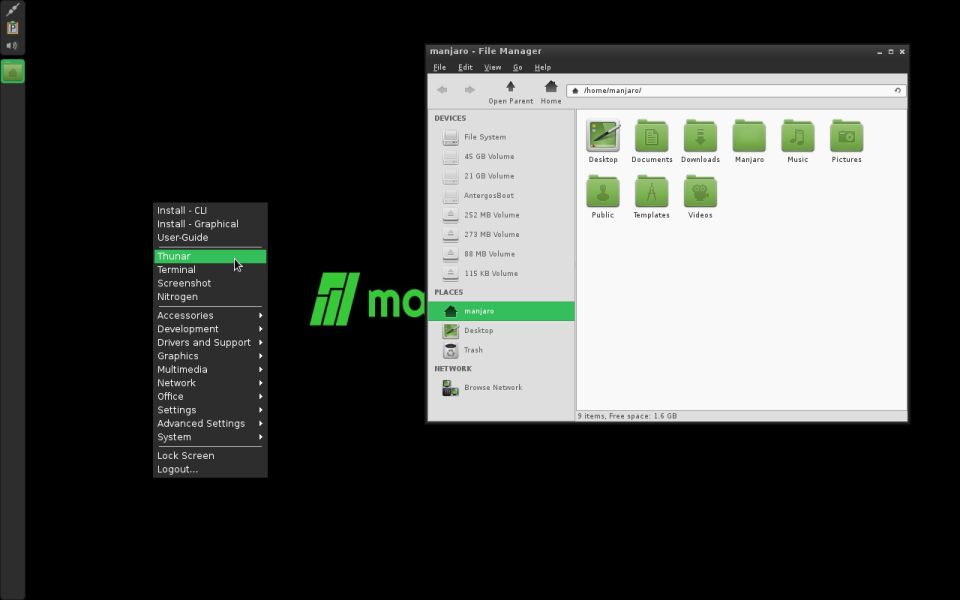
\includegraphics[scale=0.27]{manjarobox.jpg}
        \caption{Manjaro com interface gráfica Openbox}
        \label{fig:Comando ls}
    \end{figure}
\end{frame}

\begin{frame}{Manjaro}{XFCE}
 \begin{figure}[h!]
        \centering
        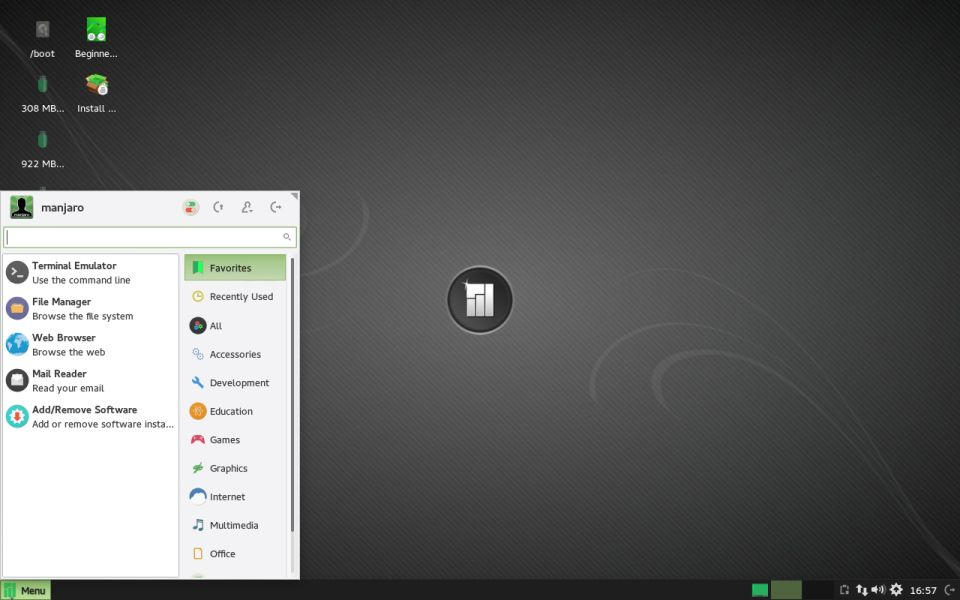
\includegraphics[scale=0.27]{manjaroXFCE.jpg}
        \caption{Manjaro com interface gráfica XFCE}
        \label{fig:Comando ls}
    \end{figure}
\end{frame}

\begin{frame}{Slackware}
    \begin{itemize}
        \item{Criada em 1991 por Linus Torvalds, o criador do Linux}
        \item{Possui um sistema de pacotes muito simples}
        \item{Usa tarballs e slackpkg como gerenciamento de pacotes}
        \item{Não possui um sistema consistente de atualizações}
        \item{É completamente livre para a escolha do usuário}
    \end{itemize}
    \begin{figure}[h!]
        \centering
        
\includegraphics[scale=0.20]{slackware.png}
    \end{figure}
\end{frame}

\begin{frame}{Slackware}{XFCE}
 \begin{figure}[h!]
        \centering
        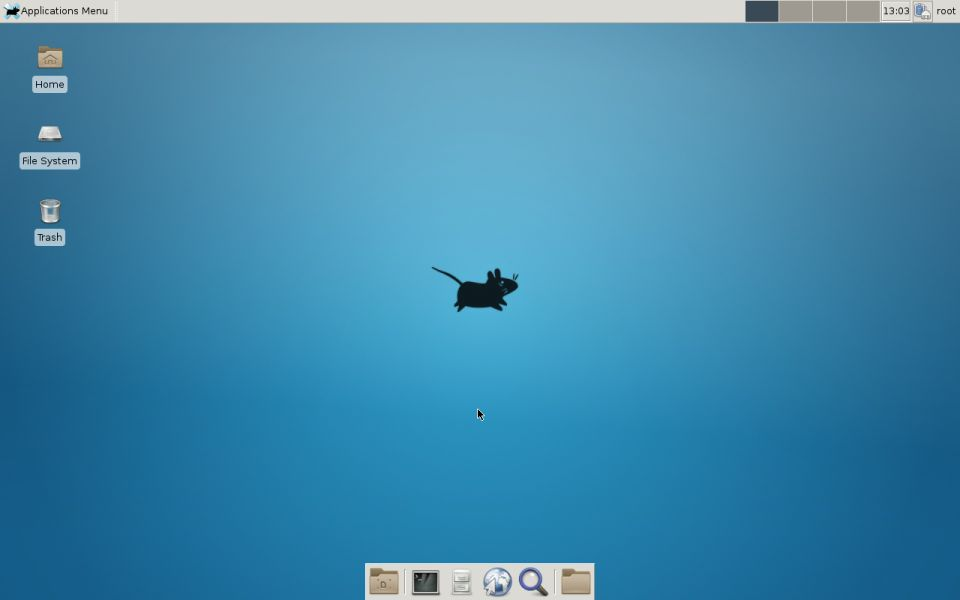
\includegraphics[scale=0.27]{slackXFCE.jpg}
        \caption{Slack com interface gráfica XFCE}
        \label{fig:Comando ls}
    \end{figure}
\end{frame}

\subsection{Minimalistas}

\begin{frame}{Arch Linux}
  \begin{itemize}
    \item{Destinada a usuários avançados, instalação completamente manual}
    \item{Sem interface gráfica por padrão}
    \item{Possui uma filosofia chamada \textbf{The Arch Way}}
    \item{Usa pacman como gerenciamento de pacotes, podendo também utilizar o AUR}
    \item{Distribuição mais atualizada entre as mais usadas}
  \end{itemize}
    \begin{figure}[h!]
        \centering
        
\includegraphics[scale=0.20]{archlinux.png}
    \end{figure}
\end{frame}

\begin{frame}{Arch Linux}{Nenhuma}
 \begin{figure}[h!]
        \centering
        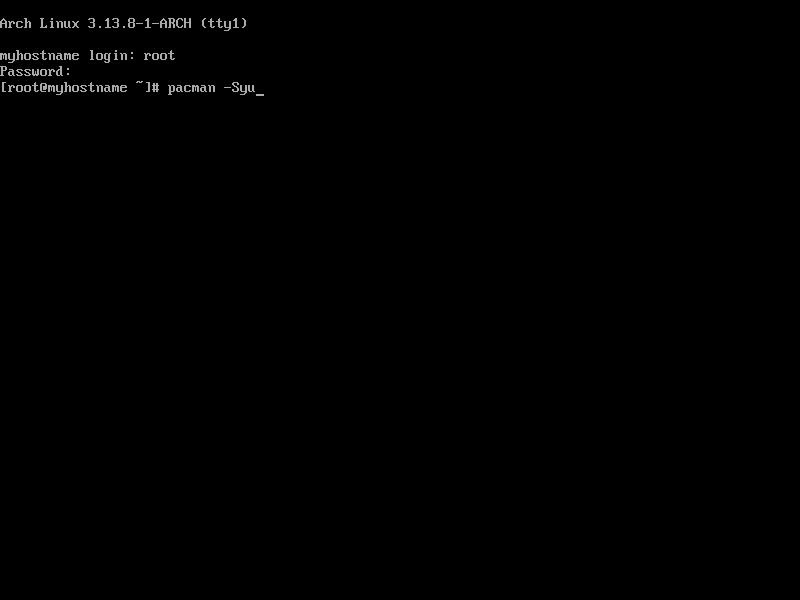
\includegraphics[scale=0.27]{archTTY.jpg}
        \caption{Arch sem interface gráfica}
        \label{fig:Comando ls}
    \end{figure}
\end{frame}

\begin{frame}{Arch Linux/Archbang}{Openbox}
 \begin{figure}[h!]
        \centering
        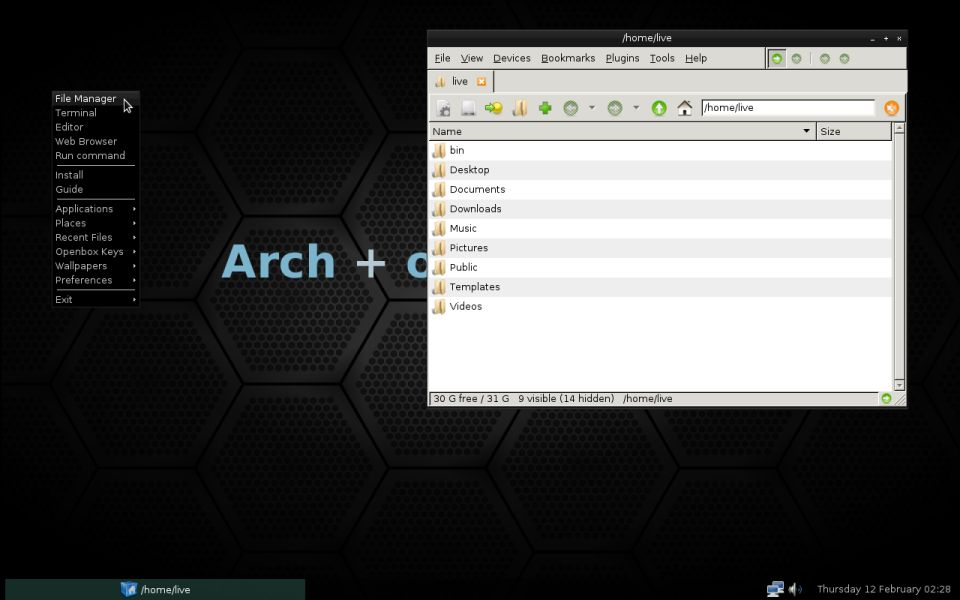
\includegraphics[scale=0.27]{archbang.jpg}
        \caption{Arch com interface gráfica Openbox}
        \label{fig:Comando ls}
    \end{figure}
\end{frame}

\begin{frame}{Gentoo}
  \begin{itemize}
    \item{Não utiliza pacotes binários, somente código fonte}
    \item{Extremamente minimalista, com instalação simplificada}
    \item{Permite personalização a níveis muito refinados}
    \item{Usa portage como gerenciamento de pacotes de código}
    \item{Muito recomendada para quem quer explorar o sistema}
  \end{itemize}
      \begin{figure}[h!]
        \centering
        
\includegraphics[scale=0.10]{gentoo.png}
    \end{figure}
\end{frame}

\begin{frame}{Gentoo}{GNOME}
 \begin{figure}[h!]
        \centering
        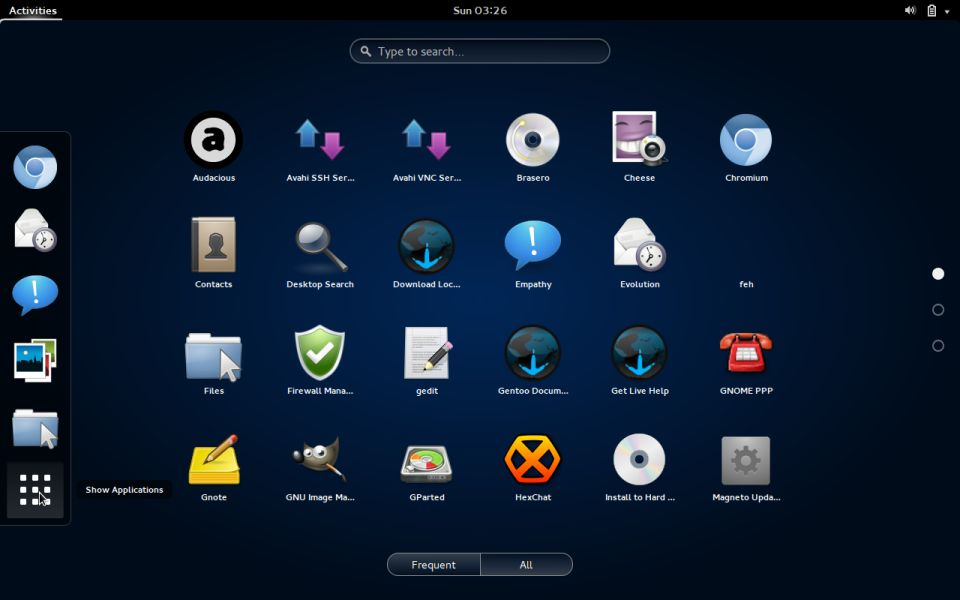
\includegraphics[scale=0.27]{gentooGNOME.jpg}
        \caption{Gentoo com interface gráfica GNOME}
        \label{fig:Comando ls}
    \end{figure}
\end{frame}

\begin{frame}{Gentoo}{KDE}
 \begin{figure}[h!]
        \centering
        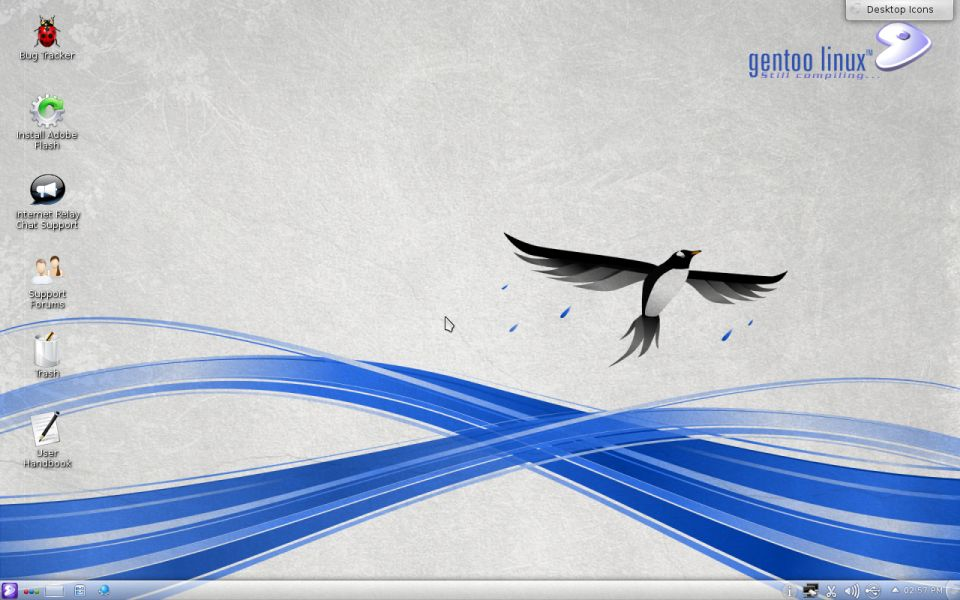
\includegraphics[scale=0.27]{gentooKDE.jpg}
        \caption{Gentoo com interface gráfica KDE}
        \label{fig:Comando ls}
    \end{figure}
\end{frame}

\section*{Sumário das distribuições}

\begin{frame}{Sumário das distribuições}
 \begin{center}
 \begin{tabular}{||r | l||} 
 \hline
 \textbf{Distribuição} & \textbf{Característica}\\ [0.5ex] 
 \hline\hline
 Ubuntu & Distribuição mais popular\\ 
 \hline
 Linux Mint & Muito amigável e fácil de usar\\
 \hline
 Fedora & Completamente livre e atualizada\\
 \hline
 Debian & Muito estável, utilizada em servidores\\
 \hline
 Manjaro & Enxuta, mas possui instalador amigável\\
 \hline
 Slackware & Livre para escolha do usuário\\
 \hline
 Arch Linux & Instalação e utilização bastante manual\\
 \hline
 Gentoo & Programas são compilados ao instalar\\
 \hline
\end{tabular}
\end{center}
\end{frame}

\begin{frame}
  This work is licensed under the Creative Commons Attribution-ShareAlike 4.0 International License. To view a copy of this license, visit \url{http://creativecommons.org/licenses/by-sa/4.0/}.
\end{frame}
\end{document}

